\chapter{2-D Convolutional Nerual Networks}
\label{3.2D_CNN}
\lhead{\emph{2-D Convolutional Neural Networks}}

During the development of the project, we have worked with four different PyEDDL versions (0.12, 0.13, 0.14 and 1.0.0) since this is a library currently in development. 3-D Convolutional Neural Networks were finally supported in PyEDDL version 1.0.0, which was released on May 27th 2021. Therefore the first CNN had to be 2-dimensionals.

This has two main drawbacks. The first one is the loss of some context information since our CNN can not analize at once a whole region of the MRI but it has to slice it, an issue inherent of working in a lower dimension. The second one is the need of having to consider also the different axles and orientations, which can be solved with data preprocessing.

\section{Data preprocessing}

For the 2-D CNN we have only used \textit{FLAIR} modality of the MRI. We first resize the \textit{FLAIR} image to $(256\times256\times256)$ so that, independently of the scanner used, the input has the same shape. After this we slice the data by the last axis. We decided this shape even when the first axis is being upsampled in all the MRI because it allows us to change the orientation or slicing axis and still having the same input shape so transfer learning techniques are possible. As a final preprocessing step we normalize each image.

No data augmentation techniques have been used since the final purpose of this project is not achieving the best accuracy (we remit to MICCAI 2016 challenge and later research works for that) but having a fair analysis and comparison of EDDL library.


%%%%%%% U-NET
\newpage
\section{U-Net}

% TODO: Number of U-Net parameters
U-Net \cite{UNET:2015} first appeared in 2015 and it quickly became the standard for biomedical image segmentation. We chose it as the model for our first approach. The network structure can be seen in the image below, the only change in the network structure in our implementation with respect to the one originally presented is that we have added batch normalization after each convolution for a better convergence and stability.

\begin{center}
\hspace*{15pt}
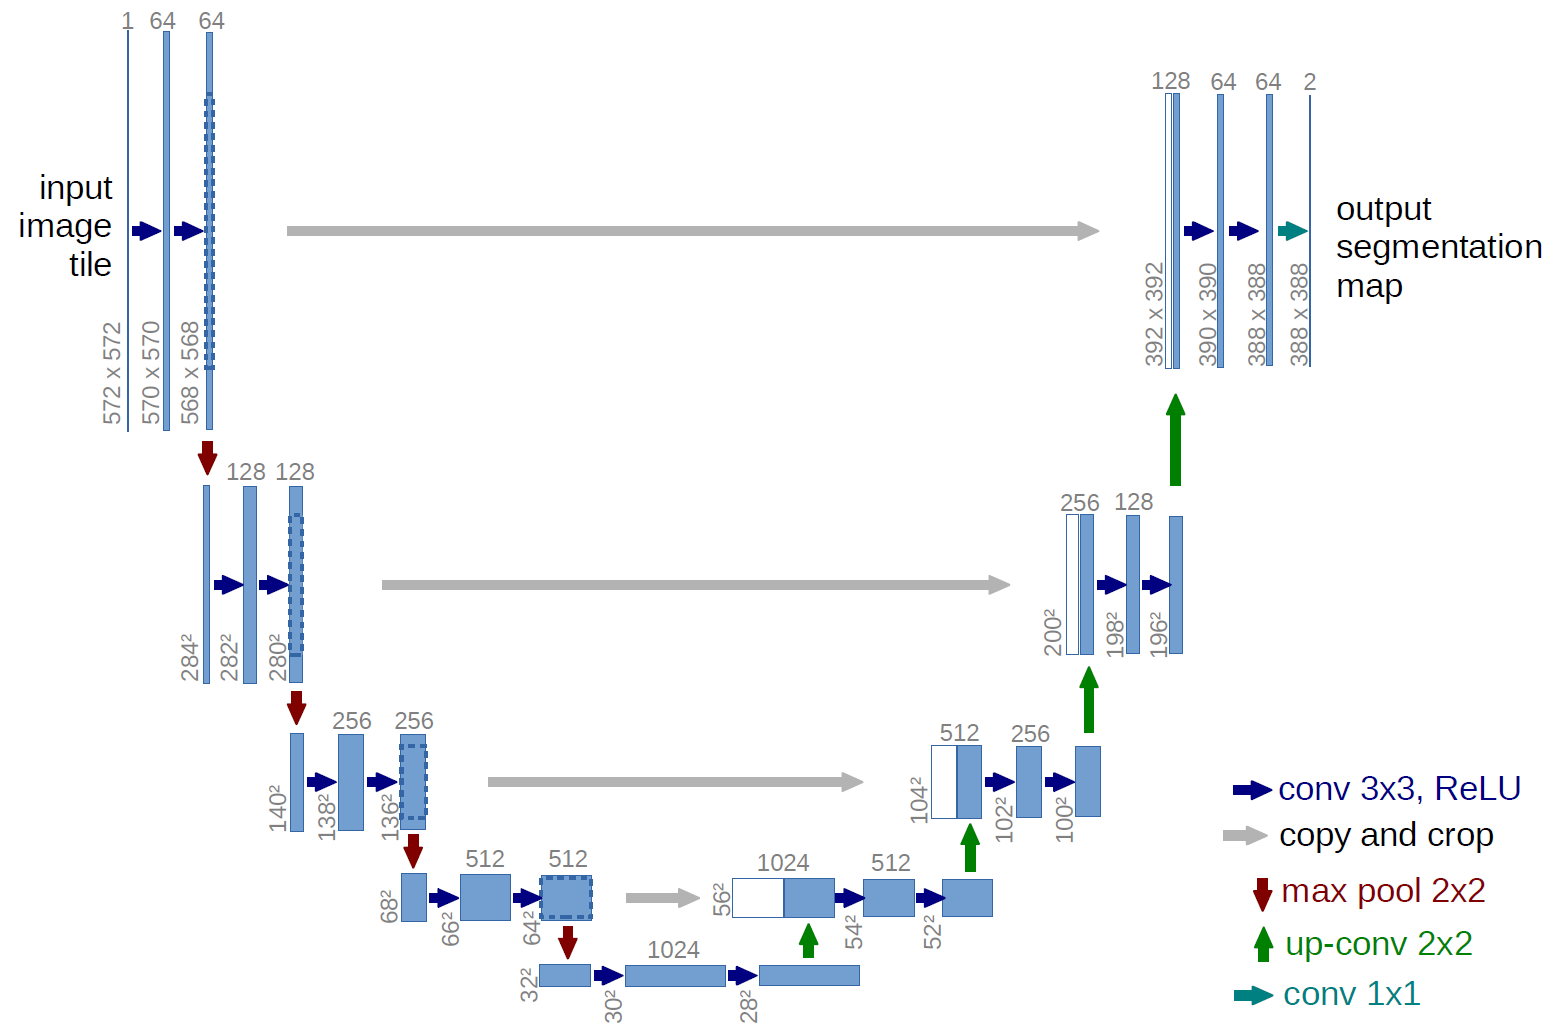
\includegraphics[width=\textwidth]{images/unet.png}
\captionof{figure}{U-Net model \cite{UNET:2015}}
\end{center}

As mentioned before, we are using \textit{Binary Cross Entropy} as loss function. In all the 2-D models we use \textit{Adam} optimizer with \textit{Learning Rate} set to 0.001 and batch size of 8 for both training and evaluation. In the case of the PyEDDL implementations, when creating the computing service (CPU or GPU) we set memory utilisation to \textit{low\_mem} so that all the models can be trained in a GPU with 16GB of memory. For a fair comparison, we maintain this value also when the target computing service is the CPU. 

We present the results of the profiling and evaluation of both a keras-tensorflow implementation and PyEDDL one (in blue and orange respectively) in the following sections:


\subsection{U-Net evaluation}

\begin{figure*}[!htb]
    \subfigure[Loss function in training per epoch]{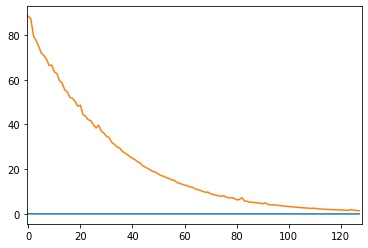
\includegraphics[width=.47\textwidth]{images/unet_images/evaluation/unet_tr_bin_ce.jpg}}\hfill
    \subfigure[Loss function in validation per epoch]{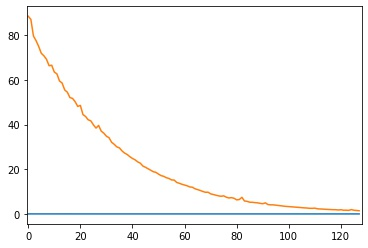
\includegraphics[width=.47\textwidth]{images/unet_images/evaluation/unet_ts_bin_ce.jpg}}
    
    \subfigure[Dice score in training per epoch]{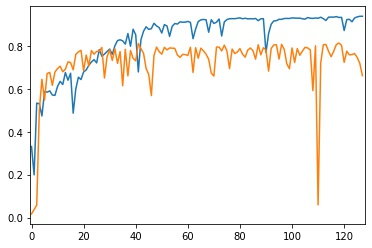
\includegraphics[width=.47\textwidth]{images/unet_images/evaluation/unet_tr_dice.jpg}\label{fig:tr943}}\hfill
    \subfigure[Dice score in validation per epoch]{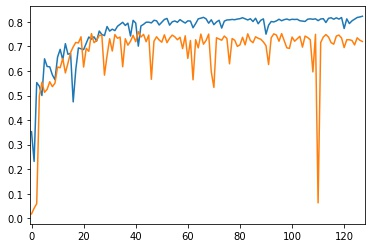
\includegraphics[width=.47\textwidth]{images/unet_images/evaluation/unet_ts_dice.jpg}\label{fig:tr1426}}
    
    \subfigure[Mean Squared Error in training per epoch]{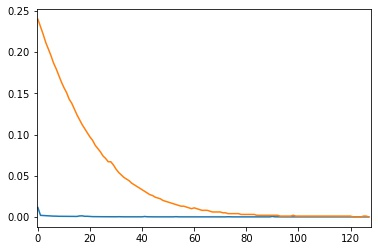
\includegraphics[width=.47\textwidth]{images/unet_images/evaluation/unet_tr_mse.jpg}}\hfill
    \subfigure[Mean Squared Error in validation per epoch]{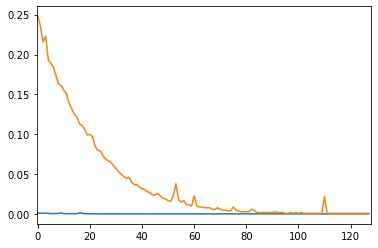
\includegraphics[width=.47\textwidth]{images/unet_images/evaluation/unet_ts_mse.jpg}}

    \subfigure[Binary Accuracy in training per epoch]{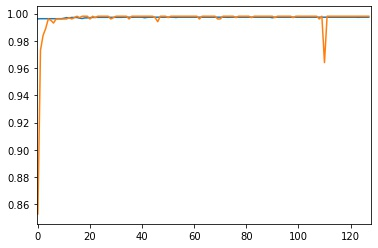
\includegraphics[width=.47\textwidth]{images/unet_images/evaluation/unet_tr_bin_acc.jpg}}\hfill
    \subfigure[Binary Accuracy in validation per epoch]{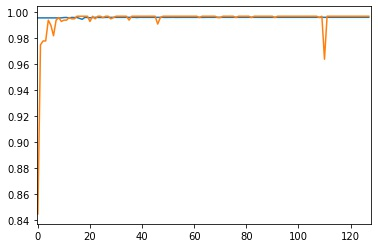
\includegraphics[width=.47\textwidth]{images/unet_images/evaluation/unet_ts_bin_acc.jpg}}
\end{figure*}

As we can see, there are huge differences in the loss function between the PyEDDL and keras-tensorflow implementations. Since these start from the very first epoch, this can be caused by the weights initialization. We can ensure this is the case by having a look to our benchmark images in the first epochs. PyEDDL U-Net predictions are shown above and keras-tensorflow model predictions below  for the benchmark image \ref{fig:tr175} at epochs 1,4,7,10 and 13. 

\begin{figure*}[!htb]
    \subfigure{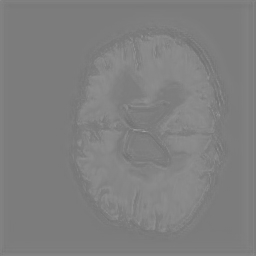
\includegraphics[width=.19\textwidth]{images/unet_images/evaluation/first_epochs/eddl/tr175_e0_pred.jpg}}\hfill
    \subfigure{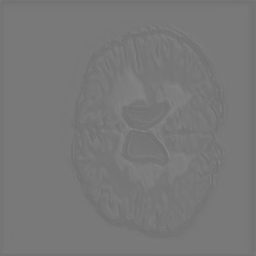
\includegraphics[width=.19\textwidth]{images/unet_images/evaluation/first_epochs/eddl/tr175_e3_pred.jpg}}\hfill
    \subfigure{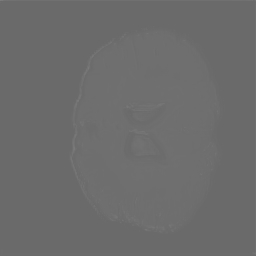
\includegraphics[width=.19\textwidth]{images/unet_images/evaluation/first_epochs/eddl/tr175_e6_pred.jpg}}\hfill
    \subfigure{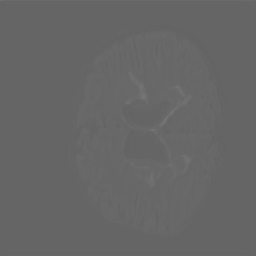
\includegraphics[width=.19\textwidth]{images/unet_images/evaluation/first_epochs/eddl/tr175_e9_pred.jpg}}\hfill
    \subfigure{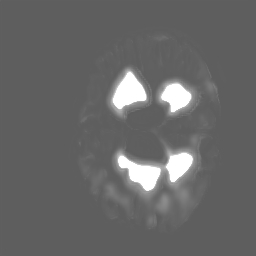
\includegraphics[width=.19\textwidth]{images/unet_images/evaluation/first_epochs/eddl/tr175_e12_pred.jpg}}
    
    \subfigure[epoch 1]{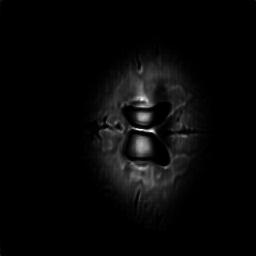
\includegraphics[width=.19\textwidth]{images/unet_images/evaluation/first_epochs/tf/tr175_e1_pred.jpg}}\hfill
    \subfigure[epoch 4]{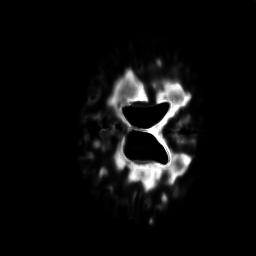
\includegraphics[width=.19\textwidth]{images/unet_images/evaluation/first_epochs/tf/tr175_e4_pred.jpg}}\hfill
    \subfigure[epoch 7]{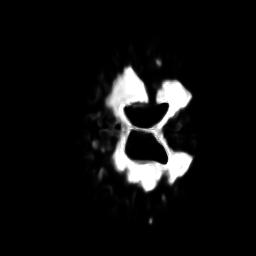
\includegraphics[width=.19\textwidth]{images/unet_images/evaluation/first_epochs/tf/tr175_e7_pred.jpg}}\hfill
    \subfigure[epoch 10]{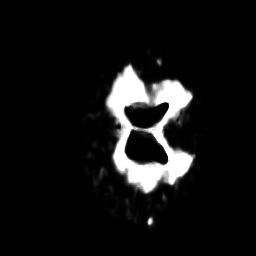
\includegraphics[width=.19\textwidth]{images/unet_images/evaluation/first_epochs/tf/tr175_e10_pred.jpg}}\hfill
    \subfigure[epoch 13]{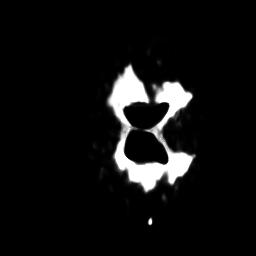
\includegraphics[width=.19\textwidth]{images/unet_images/evaluation/first_epochs/tf/tr175_e13_pred.jpg}}
\end{figure*}

We can also appreciate how the \textit{dice} metric is not so affected after few epochs. This is because, while \textit{binary cross entropy} takes in consideration the output of the network, the probability of each pixel to be part of a damaged lession, the \textit{dice} metric applies a threshold and only considers the class label assigned to that pixel. We appreciate the exact same contrast with the \textit{mean squared error} and \textit{binary accuracy}. We decided to also include them for this first evaluation to make even more clear that they are not valid metrics for our task.

There are three main appreciations when looking at the \textit{dice} score of the models. The first one and more clear is that the tensorflow (TF) model is obtaining better lesions segmentations. The second one is that, while the PyEDDL model converges, the TF model experiences a continuous improvement during the whole 128 epochs.  Finally, it's important to remark that the TF model achieves a experiences a more stable progress. Both models make missteps, i.e., epochs in which we appreaciate a drastic reduction on the \textit{dice} score, however, the TF model progres is more stable. 


Since this can be caused by the proper nature of the stochastic optimization process, even more with our small batch size, we recommend a repetition of the experiment before reaching conclusions. 

In the images below we show an explanation of the drastic reduction in the \textit{dice} score of the PyEDDL U-Net at epoch 110. Looking at the benchmark image \ref{fig:ts175}, in different stages of the training process we can appreciate how the model detects lesions in the frame of the image, being this a result of course of overfitting.

\begin{figure*}[!htb]
    \subfigure[epoch 108]{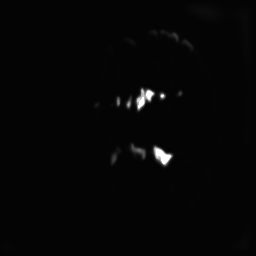
\includegraphics[width=.19\textwidth]{images/unet_images/evaluation/unstability/ts175_e108_pred.jpg}}\hfill
    \subfigure[epoch 109]{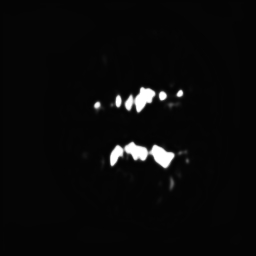
\includegraphics[width=.19\textwidth]{images/unet_images/evaluation/unstability/ts175_e109_pred.jpg}}\hfill
    \subfigure[epoch 110]{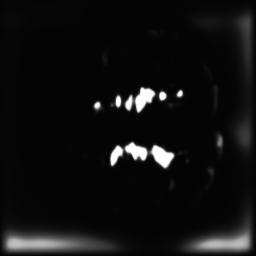
\includegraphics[width=.19\textwidth]{images/unet_images/evaluation/unstability/ts175_e110_pred.jpg}}\hfill
    \subfigure[epoch 111]{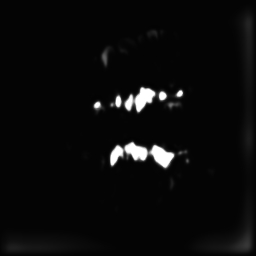
\includegraphics[width=.19\textwidth]{images/unet_images/evaluation/unstability/ts175_e111_pred.jpg}}\hfill
    \subfigure[epoch 112]{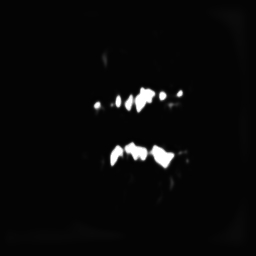
\includegraphics[width=.19\textwidth]{images/unet_images/evaluation/unstability/ts175_e112_pred.jpg}}
    
    \caption{Drastic dice score reduction at epoch 110}
\end{figure*}


\subsection{U-Net GPU profiling}
\label{U-Net GPU profile}

The profiling was done for PyEDDL 0.14.0 and TF 2.5.0 in a Tesla T-4 GPU with 16GB.

As mentioned before, we had to set the configurable memory usage parameter as \textit{low\_mem} when selecting this GPU because with a more ambitious parameter we experienced a \textit{run out of memory} error. This is a key difference. Tensorflow analyzes and evaluates the available resources at runtime and adapts to them for a faster execution and with PyEDDL we have to pre-fix a limit to the memory usage. This makes that tensorflow can extract the maximum of the available resources, using more memory and fully using the GPU while with PyEDDL we have our memory usage limited by this parameter (even when we have more memory available) and our GPU is not able to run at its full capacity. 

On the other hand, the power consumption is the same, being a bit more stable in the case of tensorflow and the GPU temperature is similar.

For the temperature profiling, which showed a very stable behaviour, we decided to profile it both when starting the execution from rest until stabilization and in the middle of the execution, in a stable middle point. This is the reason behind the differences in the train and evaluation GPU temperature profiling. The training profile \ref{unet_train_profile_temperature}, in the left, shows the the increase in temperature while the evaluation profile, in the right, shows the fluctuations in the middle of the execution. Both models behave in a very similar way being the temperature of the GPU a bit higher in the TF model.

\newpage
\begin{figure*}[!htb]
    \subfigure[Training GPU usage (\%) ]{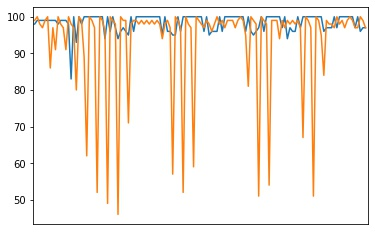
\includegraphics[width=.49\textwidth]{images/unet_images/profiling/gpu/unet_tr_gpu.jpg}}\hfill
    \subfigure[Evaluation GPU usage (\%)]{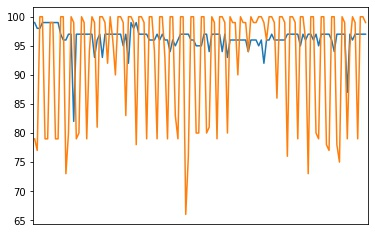
\includegraphics[width=.49\textwidth]{images/unet_images/profiling/gpu/unet_ts_gpu.jpg}}
    
    \subfigure[Training memory usage (\%)]{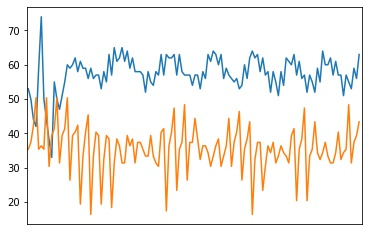
\includegraphics[width=.49\textwidth]{images/unet_images/profiling/gpu/unet_tr_memory.jpg}}\hfill
    \subfigure[Evaluation memory usage (\%)]{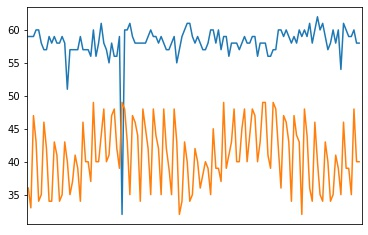
\includegraphics[width=.49\textwidth]{images/unet_images/profiling/gpu/unet_ts_memory.jpg}}
    
    \subfigure[Training power consumption (W)]{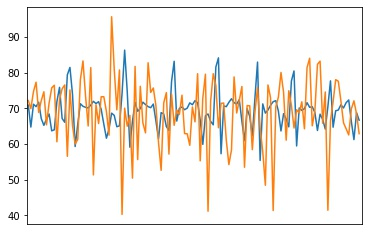
\includegraphics[width=.49\textwidth]{images/unet_images/profiling/gpu/unet_tr_power.jpg}}\hfill
    \subfigure[Evaluation power consumption (W)]{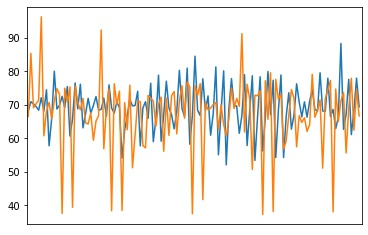
\includegraphics[width=.49\textwidth]{images/unet_images/profiling/gpu/unet_ts_power.jpg}}

    \subfigure[Training GPU temperature (ºC)]{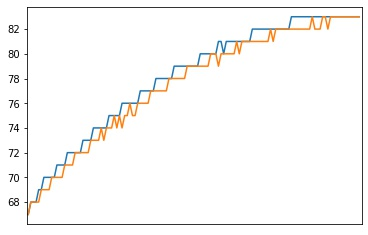
\includegraphics[width=.49\textwidth]{images/unet_images/profiling/gpu/unet_tr_temperature.jpg}\label{unet_train_profile_temperature}}\hfill
    \subfigure[Evaluation GPU temperature (ºC)]{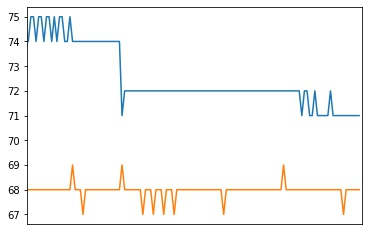
\includegraphics[width=.49\textwidth]{images/unet_images/profiling/gpu/unet_ts_temperature.jpg}}
    \caption{U-Net Tesla T-4 profile}
\end{figure*}

\newpage
\subsection{U-Net CPU profiling}
\label{U-Net CPU profiling}

The CPU profiling was done for PyEDDL 1.0.0 and TF 2.5.0 (latest stable versions when writting this report) in a server of the \textit{Embedded System Laboratory} of the \textit{École polytechnique fédérale de Lausanne}. The server counts with 80 CPUs and a total of 376GB of RAM memory.

\begin{figure*}[!htb]
    \subfigure[Training CPU usage (\%) ]{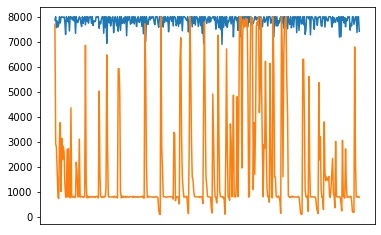
\includegraphics[width=.48\textwidth]{images/unet_images/profiling/cpu/unet_tr_CPU.jpg}}\hfill
    \subfigure[Evaluation CPU usage (\%)]{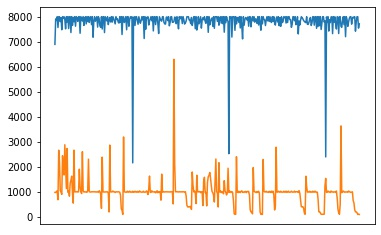
\includegraphics[width=.48\textwidth]{images/unet_images/profiling/cpu/unet_ts_CPU.jpg}}
    
    \subfigure[Training memory usage (GB)]{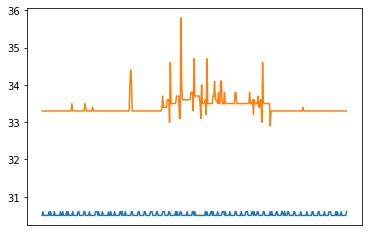
\includegraphics[width=.48\textwidth]{images/unet_images/profiling/cpu/unet_tr_memory.jpg}}\hfill
    \subfigure[Evaluation memory usage (GB)]{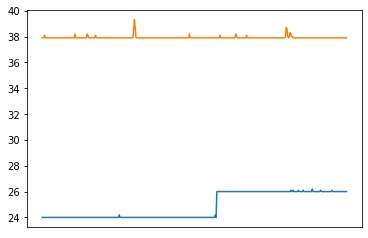
\includegraphics[width=.48\textwidth]{images/unet_images/profiling/cpu/unet_ts_memory.jpg}}
    
    \begin{comment}
    \subfigure[Training power consumption (W)]{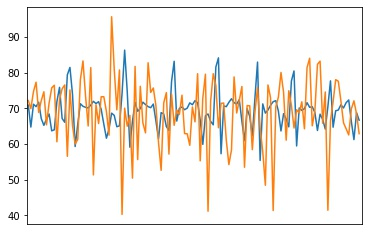
\includegraphics[width=.48\textwidth]{images/unet_images/profiling/gpu/unet_tr_power.jpg}}\hfill
    \subfigure[Evaluation power consumption (W)]{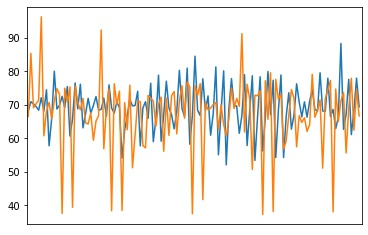
\includegraphics[width=.48\textwidth]{images/unet_images/profiling/gpu/unet_ts_power.jpg}}

    \subfigure[Training GPU temperature (ºC)]{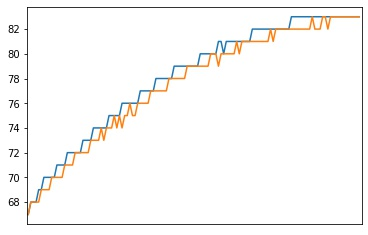
\includegraphics[width=.48\textwidth]{images/unet_images/profiling/gpu/unet_tr_temperature.jpg}}\hfill
    \subfigure[Evaluation GPU temperature (ºC)]{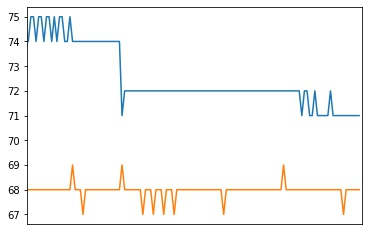
\includegraphics[width=.48\textwidth]{images/unet_images/profiling/gpu/unet_ts_temperature.jpg}}
    \end{comment}
\end{figure*}


For the profile we again set the memory parameter of the PyEDDL CPU computing service to \textit{low\_mem} and we also set \textit{th=-1} so that we allow PyEDDL to use all the available CPUs, configuring TF also in the same way. 

At this point, the data speaks for itself. There are evident differences in the resources management. While TF is able to fully use all the CPUs with a reasonable cost of memory, PyEDDL is only able to use around one eigth of the computation power, the equivalent of 10 CPUs, and with a much higher memory cost. During training we can appreciate some peaks of CPU utilization reaching all the server capacity but these are unstable.

As in previous versions of PyEDDL, TF offers a better memory consumption and resources management. These are are two of the main niches of improvement of this library in development.




%%%%%%% DOUBLE U-NET
\newpage
\section{Double U-Net}

The second 2-D CNN implemented to address the problem of MS lesion segmentation was the Double U-Net \cite{DOUBLE_UNET:2020}. It appeared last year and, following the encode-decode logic of the U-Net model, duplicates this adopting in its structure some networks which have proven to be useful or a significative improvement in several tasks, as the VGG-19 and the ASPP. % TODO: Cite VGG-19 and ASPP
As U-Net, it's a fully CNN, it processes the image in its totality. 

The original model structure can be seen below. The only modifications done with respect to it is that our output is \textit{output2} and that we had to add concatenations of a layer with itself at the beggining of the \textit{Network 2} because PyEDDL only supports multiplication of tensors with the exact same shape.

\begin{center}
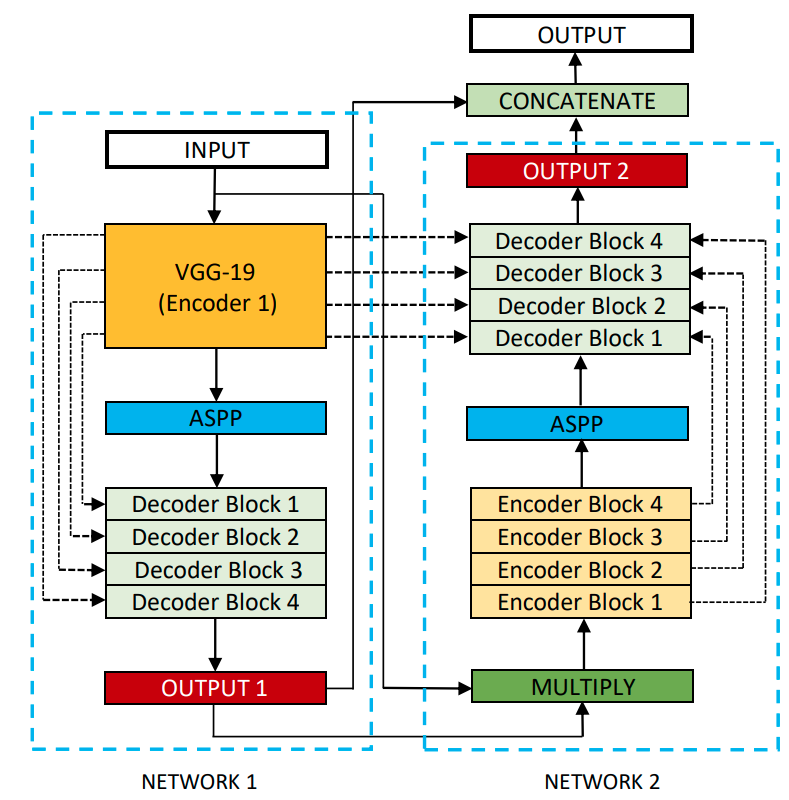
\includegraphics[width=\textwidth]{images/double_unet.png}
\captionof{figure}{Double U-Net model \cite{DOUBLE_UNET:2020}}
\end{center}
% TODO: Double U-Net
% -> PyEDDL
% -> Tensorflow
%
% -> Dice scores
% -> Profiles
% -> Network output

\newpage
\subsection{Double U-Net evaluation}

\begin{figure*}[!htb]
    \subfigure[Loss function in training per epoch]{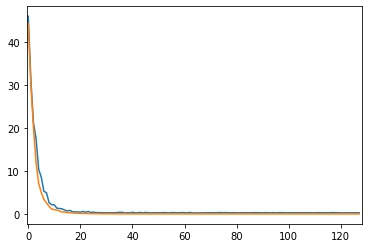
\includegraphics[width=.47\textwidth]{images/double_unet_images/evaluation/double_unet_tr_bin_ce.jpg}}\hfill
    \subfigure[Loss function in validation per epoch]{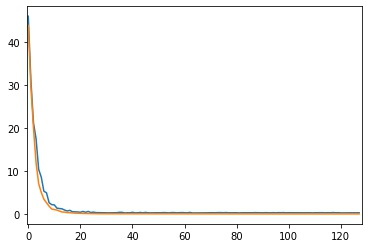
\includegraphics[width=.47\textwidth]{images/double_unet_images/evaluation/double_unet_ts_bin_ce.jpg}}
    
    \subfigure[Dice score in training per epoch]{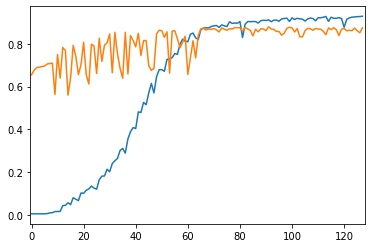
\includegraphics[width=.47\textwidth]{images/double_unet_images/evaluation/double_unet_tr_dice.jpg}}\hfill
    \subfigure[Dice score in validation per epoch]{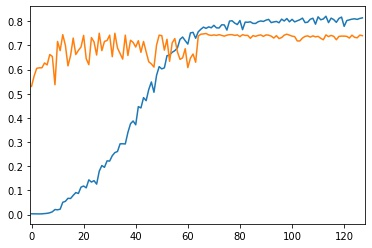
\includegraphics[width=.47\textwidth]{images/double_unet_images/evaluation/double_unet_ts_dice.jpg}}
    \begin{comment}
    \subfigure[Mean Squared Error in training per epoch]{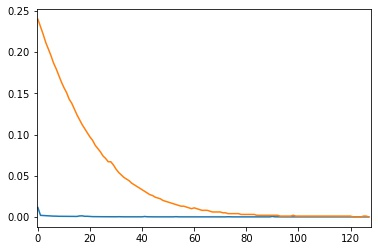
\includegraphics[width=.47\textwidth]{images/unet_images/evaluation/unet_tr_mse.jpg}}\hfill
    \subfigure[Mean Squared Error in validation per epoch]{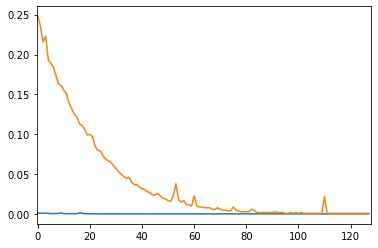
\includegraphics[width=.47\textwidth]{images/unet_images/evaluation/unet_ts_mse.jpg}}

    \subfigure[Binary Accuracy in training per epoch]{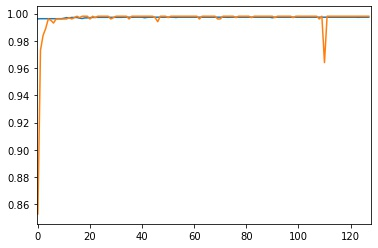
\includegraphics[width=.47\textwidth]{images/unet_images/evaluation/unet_tr_bin_acc.jpg}}\hfill
    \subfigure[Binary Accuracy in validation per epoch]{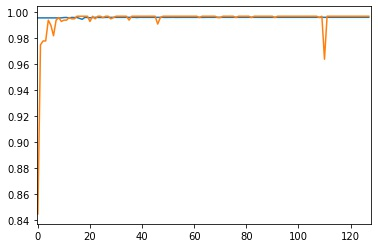
\includegraphics[width=.47\textwidth]{images/unet_images/evaluation/unet_ts_bin_acc.jpg}}
    \end{comment}
    
\end{figure*}

\vspace{-7pt}
We can appreciate again how the TF model follows a continuous improvement while the PyEDDL model stabilizes with a lower \textit{dice} score. It's remarcable however how slow is the increase of the quality of the segmentations of the TF model. Again, this is due to weights initialization. Looking at the benchmark image \ref{fig:tr1426} can appreciate how the PyEDDL model (above) starts from a closer initialization to the output mask and aproximates to this much faster than the TF model (below).

\begin{figure*}[!htb]
    \subfigure{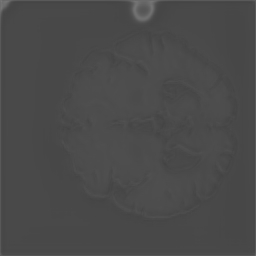
\includegraphics[width=.19\textwidth]{images/double_unet_images/evaluation/first_epochs/eddl/tr1426_e0_pred.jpg}}\hfill
    \subfigure{\includegraphics[width=.19\textwidth]{images/double_unet_images/evaluation/first_epochs/eddl/tr1426_e3_pred.jpg}}\hfill
    \subfigure{\includegraphics[width=.19\textwidth]{images/double_unet_images/evaluation/first_epochs/eddl/tr1426_e6_pred.jpg}}\hfill
    \subfigure{\includegraphics[width=.19\textwidth]{images/double_unet_images/evaluation/first_epochs/eddl/tr1426_e9_pred.jpg}}\hfill
    \subfigure{\includegraphics[width=.19\textwidth]{images/double_unet_images/evaluation/first_epochs/eddl/tr1426_e12_pred.jpg}}
    
    \subfigure[epoch 1]{\includegraphics[width=.19\textwidth]{images/double_unet_images/evaluation/first_epochs/tf/tr1426_e1_pred.jpg}}\hfill
    \subfigure[epoch 4]{\includegraphics[width=.19\textwidth]{images/double_unet_images/evaluation/first_epochs/tf/tr1426_e4_pred.jpg}}\hfill
    \subfigure[epoch 7]{\includegraphics[width=.19\textwidth]{images/double_unet_images/evaluation/first_epochs/tf/tr1426_e7_pred.jpg}}\hfill
    \subfigure[epoch 10]{\includegraphics[width=.19\textwidth]{images/double_unet_images/evaluation/first_epochs/tf/tr1426_e9_pred.jpg}}\hfill
    \subfigure[epoch 13]{\includegraphics[width=.19\textwidth]{images/double_unet_images/evaluation/first_epochs/tf/tr1426_e12_pred.jpg}}
\end{figure*}



\newpage
\subsection{Double U-Net GPU profiling}

\begin{figure*}[!htb]
    \subfigure[Training GPU usage (\%) ]{\includegraphics[width=.48\textwidth]{images/double_unet_images/profiling/gpu/double_unet_tr_gpu.jpg}}\hfill
    \subfigure[Evaluation GPU usage (\%)]{\includegraphics[width=.48\textwidth]{images/double_unet_images/profiling/gpu/double_unet_ts_gpu.jpg}}
    
    \subfigure[Training memory usage (\%)]{\includegraphics[width=.48\textwidth]{images/double_unet_images/profiling/gpu/double_unet_tr_memory.jpg}}\hfill
    \subfigure[Evaluation memory usage (\%)]{\includegraphics[width=.48\textwidth]{images/double_unet_images/profiling/gpu/double_unet_ts_memory.jpg}}
    
    \subfigure[Training power consumption (W)]{\includegraphics[width=.48\textwidth]{images/double_unet_images/profiling/gpu/double_unet_tr_power.jpg}}\hfill
    \subfigure[Evaluation power consumption (W)]{\includegraphics[width=.48\textwidth]{images/double_unet_images/profiling/gpu/double_unet_ts_power.jpg}}

    \subfigure[Training GPU temperature (ºC)]{\includegraphics[width=.48\textwidth]{images/double_unet_images/profiling/gpu/double_unet_tr_temperature.jpg}}\hfill
    \subfigure[Evaluation GPU temperature (ºC)]{\includegraphics[width=.48\textwidth]{images/double_unet_images/profiling/gpu/double_unet_ts_temperature.jpg}}
    \caption{Double U-Net GPU profile}
\end{figure*}

The profile was done under the same conditions than \ref{U-Net GPU profile} and the results extracted are totally analogous to the ones presented for the U-Net case, with the exception of the memory usage, where the Double U-Net requires a little more memory (less than 300MB in average). This reaffirms our previous conclusions about the comparison of PyEDDL and TF so for avoiding repetition we remit to \ref{U-Net GPU profile} and we won't further discuss it.

\vspace{-7pt}
\subsection{Double U-Net CPU profiling}

Double U-Net CPU profiling was done under the exact same conditions than \ref{U-Net CPU profiling} the results we obtained are consistent with the U-net profile. We again see huge differences in the ratio memory-cpu usage, being PyEDDL again unable to distribute the training or evaluation process in a more efficient way to take advantage of all hardware resources. 

The CPU utilization is the same as in the U-Net, with the PyEDDL model around the compute capacity of 10 CPUs but, in this case, differences in memory usage between the U-Net and the Double U-Net model in the PyEDDL model are significant, around 9GB more in the Double U-Net. As this is not the case in the TF library we can't conclude that Double U-Net is a more memory-consuming model itself.
\vspace{-5pt}

\begin{figure*}[!htb]
    \subfigure[Training CPU usage (\%) ]{\includegraphics[width=.48\textwidth]{images/double_unet_images/profiling/cpu/double_unet_tr_CPU.jpg}}\hfill
    \subfigure[Evaluation CPU usage (\%)]{\includegraphics[width=.48\textwidth]{images/double_unet_images/profiling/cpu/double_unet_ts_CPU.jpg}}
    
    \subfigure[Training memory usage (GB)]{\includegraphics[width=.48\textwidth]{images/double_unet_images/profiling/cpu/double_unet_tr_memory.jpg}}\hfill
    \subfigure[Evaluation memory usage (GB)]{\includegraphics[width=.48\textwidth]{images/double_unet_images/profiling/cpu/double_unet_ts_memory.jpg}}
    
    \begin{comment}
    \subfigure[Training power consumption (W)]{\includegraphics[width=.48\textwidth]{images/unet_images/profiling/gpu/unet_tr_power.jpg}}\hfill
    \subfigure[Evaluation power consumption (W)]{\includegraphics[width=.48\textwidth]{images/unet_images/profiling/gpu/unet_ts_power.jpg}}

    \subfigure[Training GPU temperature (ºC)]{\includegraphics[width=.48\textwidth]{images/unet_images/profiling/gpu/unet_tr_temperature.jpg}}\hfill
    \subfigure[Evaluation GPU temperature (ºC)]{\includegraphics[width=.48\textwidth]{images/unet_images/profiling/gpu/unet_ts_temperature.jpg}}
    \end{comment}
\end{figure*}

%%%%%%% COMPARISON
\newpage
\section{Comparison}

We provide the result of our experiments so that both models and libraries can be compared. Given the amount of non-deterministic factors involved, as the weights initialization and the intrinsic randomness of the stochastic optimization processes, we encourage anybody with the intention of using this data to replicate several times the experiment to obtain more accurate values.

\vspace{0.75cm}


\begin{table}[!htb]
\centering
\begin{tabular}{l|l|l|}
\cline{2-3}
\multicolumn{1}{c|}{\textbf{U-NET}}                              & \multicolumn{1}{c|}{\textbf{PyEDDL}} & \multicolumn{1}{c|}{\textbf{Tensorflow}} \\ \hline
\multicolumn{1}{|l|}{Trainable parameters}                       &             31,060,241                         &                            31,031,685              \\ \hline
\multicolumn{1}{|l|}{Non-trainable parameters}                   &               0                       &                                    0      \\ \hline

\multicolumn{1}{|l|}{Epoch training time (CPU)}                        &                 $\approx$ 10h                     &                                        $\approx$ 32min  \\ \hline
\multicolumn{1}{|l|}{Evaluation time (CPU)}                            &                      $\approx$ 70min                &                                        $\approx$ 1min  \\ \hline
\multicolumn{1}{|l|}{Best dice score in training}                &                   0.81                   &                                      0.93    \\ \hline
\multicolumn{1}{|l|}{Best dice score in validation}              &                   0.76                   &                                      0.82    \\ \hline
\multicolumn{1}{|l|}{GPU utilization in training (avg \%)}          &                   97.30                   &                                     98.54     \\ \hline
\multicolumn{1}{|l|}{GPU memory utilization in training (avg \%)}   &                49.84                      &                                  57.86        \\ \hline
\multicolumn{1}{|l|}{CPU utilization in training (avg \%)}          &             1791.22                         &                             7834.15             \\ \hline
\multicolumn{1}{|l|}{CPU memory utilization in training (avg GB)}   &               33.39                       &                                 30.52         \\ \hline
\multicolumn{1}{|l|}{GPU utilization in validation (avg \%)}        &                92.74                      &                                  96.26        \\ \hline
\multicolumn{1}{|l|}{GPU memory utilization in validation (avg \%)} &                   41.01                   &                                     58.31     \\ \hline
\multicolumn{1}{|l|}{CPU utilization in validation (avg \%)}        &                   1012.64                   &                                   7795.93       \\ \hline
\multicolumn{1}{|l|}{CPU memory utilization in validation (avg GB)} &                   37.91                   &                                     25.16     \\ \hline
\end{tabular}
\end{table}

\vspace{1cm}

\begin{table}[!htb]
\centering
\begin{tabular}{l|l|l|}
\cline{2-3}
\multicolumn{1}{c|}{\textbf{DOUBLE U-NET}}                              & \multicolumn{1}{c|}{\textbf{PyEDDL}} & \multicolumn{1}{c|}{\textbf{Tensorflow}} \\ \hline
\multicolumn{1}{|l|}{Trainable parameters}                       &               29,320,226                       &                              29,288,546            \\ \hline
\multicolumn{1}{|l|}{Non-trainable parameters}                   &                   7,296                   &                                     7,296     \\ \hline
\multicolumn{1}{|l|}{Epoch training time (CPU)}                        &             $\approx$ 13h                         &                                    $\approx$ 46min      \\ \hline
\multicolumn{1}{|l|}{Evaluation time (CPU)}                            &             $\approx$ 85min                         &                                    $\approx$ 1.5min      \\ \hline
\multicolumn{1}{|l|}{Best dice score in training}                &                  0.88                    &                                     0.92     \\ \hline
\multicolumn{1}{|l|}{Best dice score in validation}              &                  0.75                    &                                     0.82     \\ \hline
\multicolumn{1}{|l|}{GPU utilization in training (avg \%)}          &                 93.67                     &                                   98.22       \\ \hline
\multicolumn{1}{|l|}{GPU memory utilization in training (avg \%)}   &                  39.50                    &                                    62.21      \\ \hline
\multicolumn{1}{|l|}{CPU utilization in training (avg \%)}          &                   2000.80                   &                                   7778.40       \\ \hline
\multicolumn{1}{|l|}{CPU memory utilization in training (avg GB)}   &                   40.43                   &                                     29.90     \\ \hline
\multicolumn{1}{|l|}{GPU utilization in validation (avg \%)}        &                  96.65                    &                                    96.62      \\ \hline
\multicolumn{1}{|l|}{GPU memory utilization in validation (avg \%)} &                   45.08                   &                                     63.72     \\ \hline
\multicolumn{1}{|l|}{CPU utilization in validation (avg \%)}        &                  1134.80                    &                                  7810.52        \\ \hline
\multicolumn{1}{|l|}{CPU memory utilization in validation (avg GB)} &                   46.62                   &                                     24.63     \\ \hline
\end{tabular}
\end{table}
